\documentclass{sigchi}

% Use this command to override the default ACM copyright statement (e.g. for preprints). 
% Consult the conference website for the camera-ready copyright statement.
\toappear{
	Submitted for review.
}

% Arabic page numbers for submission. 
% Remove this line to eliminate page numbers for the camera ready copy
\pagenumbering{arabic}


% Load basic packages
\usepackage{balance}  % to better equalize the last page
\usepackage{graphics} % for EPS, load graphicx instead
\usepackage{times}    % comment if you want LaTeX's default font
\usepackage{url}      % llt: nicely formatted URLs

% llt: Define a global style for URLs, rather that the default one
\makeatletter
\def\url@leostyle{%
  \@ifundefined{selectfont}{\def\UrlFont{\sf}}{\def\UrlFont{\small\bf\ttfamily}}}
\makeatother
\urlstyle{leo}


% To make various LaTeX processors do the right thing with page size.
\def\pprw{8.5in}
\def\pprh{11in}
\special{papersize=\pprw,\pprh}
\setlength{\paperwidth}{\pprw}
\setlength{\paperheight}{\pprh}
\setlength{\pdfpagewidth}{\pprw}
\setlength{\pdfpageheight}{\pprh}

% Make sure hyperref comes last of your loaded packages, 
% to give it a fighting chance of not being over-written, 
% since its job is to redefine many LaTeX commands.
\usepackage{hyperref}
\hypersetup{
pdftitle={Authorized Power Outlet},
pdfauthor={LaTeX},
pdfkeywords={SIGCHI, proceedings, archival format},
bookmarksnumbered,
pdfstartview={FitH},
colorlinks,
citecolor=black,
filecolor=black,
linkcolor=black,
urlcolor=black,
breaklinks=true,
}

% create a shortcut to typeset table headings
\newcommand\tabhead[1]{\small\textbf{#1}}


% End of preamble. Here it comes the document.
\begin{document}

\title{Authorized Power Outlet}

\numberofauthors{3}
\author{
  \alignauthor Ryan Fahsel\\
    \affaddr Georgia Institute of Technology\\
%    \affaddr{Address}\\
    \email ryan.fahsel@gatech.edu\\
%    \affaddr{Optional phone number}
  \alignauthor Colin Gray\\
    \affaddr Georgia Institute of Technology\\
%    \affaddr{Address}\\
    \email colin.gray@gatech.edu\\
%    \affaddr{Optional phone number}    
  \alignauthor Ramya Ramakrishnan\\
    \affaddr Georgia Institute of Technology\\
%    \affaddr{Address}\\
    \email rramakrishnan3@gatech.edu\\
%    \affaddr{Optional phone number}
}

\maketitle

\begin{abstract}
This project explores opportunities to improve the current implementation of authenticated power outlets. The motivation for this research is to increase scalability, marketability and accessibility.  Previous studies have looked into using wireless technology to control outlets. One such example is the Belkin WeMo; however, these devices have not had a authentication focus. In our work, improvements include implementing a Personal Area Network of wireless outlet receptacles, smaller form factor, user device tracking system, automatic time out, and a non-NFC form of authentication in the form of QR codes, which increases access to this new technology. From this project we have learned that there are many additional roles that authorized power outlets can play, and there are some usability improvements that can be implemented to help the technology better assimilate into society. In future work, we hope to get farther in the process of reducing the form factor.
\end{abstract}

\keywords{
	NFC; RFID; Authorization.
%	\textcolor{red}{Mandatory section to be included in your final version.}
}

\category{K.6.5.}{}{}


\terms{
	Human Factors; Security. 
}

%See list of the limited ACM 16 terms in the
%instructions and additional information:
%\url{http://www.sheridanprinting.com/sigchi/generalterms.htm}.
%\textcolor{red}{Optional section to be included in your final version.}

\section{Introduction}

\subsection {Project Description}
The goal of this project is to improve upon existing authenticated power outlets. While the work done by Fahsel, Gray, and Ramakrishnan proved that this technology works with their NFCOutlet, it lacks scalability and marketability [2]. This project sets out to add features to authenticated power outlets to allow them to be more easily implemented in industry and society as well as explore what other major industry responsibilities can be done by authorized power outlets.

\subsection {Motivation}
The motivation of this project was to take a large bulky prototype and see if it was possible to take the work done in NFCOutlet and make it smaller, more accessible, and more useful. Large amounts of data has proved itself to be a valuable asset in industry time and time again. Because a request has to be sent to a server from an authenticated user every time someone wants to power on an outlet, this has the potential to be a source for massive amounts of data. This has numerous applications; however, one specific application is in manufacturing. Manufactures are looking for new ways to track what employee is using what equipment and for how long and ways to regulate equipment use to only trained employees. Currently, many manufacturers use physical keys to authenticate to machines; however employees often leave these in machines and leave the machines unattended [3,7]. This research will try to find a way to address these issues using authenticated power outlets. 

Another potential use is in the home [3,7]. The original NFCOutlet was very large and not practical for the home; thus, another goal of this research is to make the device smaller. If this research can find a way to do so, then these devices might become more commonplace in homes. In order for this type of device to become more ubiquitous in the home; however, the authentication medium must be one readily available to the user. While NFC is being built into more and more phones, there are people without these phones who may not be able to use this technology [2]. This research sets out to see if there is another medium of authentication that could be used by subjects who may not have NFC capabilities. 

Lastly, with more and more research being done on wireless solutions and personal area networks, our research has been motivated to explore possible ways to eliminate the need for an ethernet connection for every authorized power outlet [3]. This could result in much greater scalability. If this research can achieve wireless connectivity, it could allow for authorized power outlets to become as commonplace as any other consumer device that uses a wireless connection.

\section{Previous/Related Work}
We conducted previous work in this area to determine the effectiveness of using NFC for authorization. The results of this research were that the the NFC technology embedded in phones was an effective way to transmit the credentials of users. Each tool in the system was associated with an NFC sticker that was simple to use and worked well with the NFC embedded in the mobile device. The system could be easily implemented in a larger scale because phones with embedded NFC have become much more common and NFC stickers can be easily incorporated [2].

Previous studies have also looked into using wireless networks to control some system. A study looked at the Belkin WeMo switch as a way to wirelessly turn a light bulb on and off. So, instead of using the standard switch to turn on a bulb, the researchers sent messages using the internet so that it could be switched on wirelessly. This is similar to the wireless networking we would like to include in NFCOutlet [3]. 

One study designed and implemented a wireless power outlet system in the home so that the outlets can be automatically controlled. It used a ZigBee radio as an actuator node for remote control. The results of the research were that this system was rather simple and flexible and was able to control many of the appliances in the house [7].

Another study analyzed how wireless devices can be used for controlling generic systems. In this work, input was received from a power source and multiple wireless devices in the system. A processor received many of these signals from the network and transmitted them to the output controller. This controller then used these signals to decide whether or not to provide power to some set of equipment [5].

In another research work, Singhee designed a system that could intelligently exchange information between a system and its environment. He used the Nintendo Wii Remote as a way to transmit LED information. The results of the research was that a complex system was created with effective information flow. Although for the purposes of our work proposed here, we plan to have a simpler system [6].

Several studies have also tracked usage of equipment, as we plan to do in this project. In one study, equipment usage was tracked in the hospital where RFID technology was being used to keep track of patients. The tracking was effective in preventing theft in the hospital [8]. Similarly, in this project, we hope to track equipment usage, as that will provide more information about our system and its users.

As a whole, the previous work in this field has looked into using wireless networks for various applications, such as controlling home appliances and transmitting LED information. We hope to use similar wireless systems to control the network of outlets that we plan to use for authorization. Studies have also analyzed equipment usage, and we hope to implement a similar system to track usage of authorized tools.

\section{Our Work}

\subsection {Resources}
There were four main components to this project:  Android devices, a webserver,  an outlet receptacle, and a base station. Additionally, we needed to print specific QR codes to access and authenticate each connected device.
\begin{itemize}
\item Android devices: A Nexus 7 which is NFC enabled and a non-NFC enabled android phone was used
\item Webserver: Georgia Tech offers free hosting to all students. A Fedora powered webserver with PHP, Python, and MySQL access was used.
\item Outlet Receptacle 1: A wall wart with a printed circuit board that takes wireless input via a ZigBee and either activates or deactivates the attached outlet. 
\item Outlet Receptacle 2: A large box with a circuit that takes wireless input via a ZigBee and either activates or deactivates the attached outlet. 
\item Base Station: Contains a RaspberryPi connected to a ZigBee interfaced via a serial connection, allowing for the base station to communicate with the outlet receptacles.
\end{itemize}
\subsection{Implementation}
For this specific research, we implemented the authorized power outlet system in a prototyping lab consisting of several tools that require training or supervision to use; therefore authenticated connected devices are referred to as tools in this scenario. The following implementation will be referred to in the context of this application.

For implementing the tracking system, a webpage was created to allow a user to check each tool’s usage. PHP was used for the server-side web development, and MySQL was used to query the database and obtain information about the users and tools. There was a table that stored users and their ids and another table for the tools. Finally, there was a permissions table that stored all of the users and the tools they are authorized to use. It also contained a count of how many times that user has used that tool. The main page showed the total number of times each tool was used. Then, if any tool was selected, a table was displayed to show how many times each user had used that particular tool. These numbers came from a database that stored all the authorized users and tools in the system. This tracking system can be very useful in monitoring usage statistics and can help decide what new tools are needed.

To  further increase accessibility we implemented scanner in the Android application to read QR codes. We were able to integrate a popular open source android scanner called “Zebra Crossing” into the current Android application. Readily available QR code generators were used create QR codes specific to each individual tool, similar to NFC tags. 

To implement a wireless infrastructure, this research created a base station client architecture. This architecture is composed of a base station that interprets data from a database and sends on and off signals to remote outlets accordingly. The relationship of base stations to clients is 1-N. 

To implement a base station to communicate with the authorized outlet, a single board computer known as a Raspberry Pi ran a Java program that continually checked a MySQL database. This database held information about which devices should be powered on and which devices should not be powered on. These values were changed via the Android application discussed in the work done by Fahsel, Colin and Ramakrishnan [2]. The Java program parsed the response from the database, and if the status of a device changed, a broadcast would be sent out via a ZigBee module to a remote outlet, enabling or disabling the outlet.  

To implement the remote power outlet, the same box is used that was used in work done by  Fahsel, Colin and Ramakrishnan with one slight change [2]. The Arduino was replaced with a ZigBee module. This allowed the outlet to listen to instructions from the base station. In the course of the research, a printed circuit board was designed on EAGLE CAD to be housed in a wall wart; however, because of lack of proper equipment, the printed circuit board was never realized. See appendix A for EAGLE CAD printed circuit board design and appendix B for wall wart.

\begin{figure}[!h]
\centering
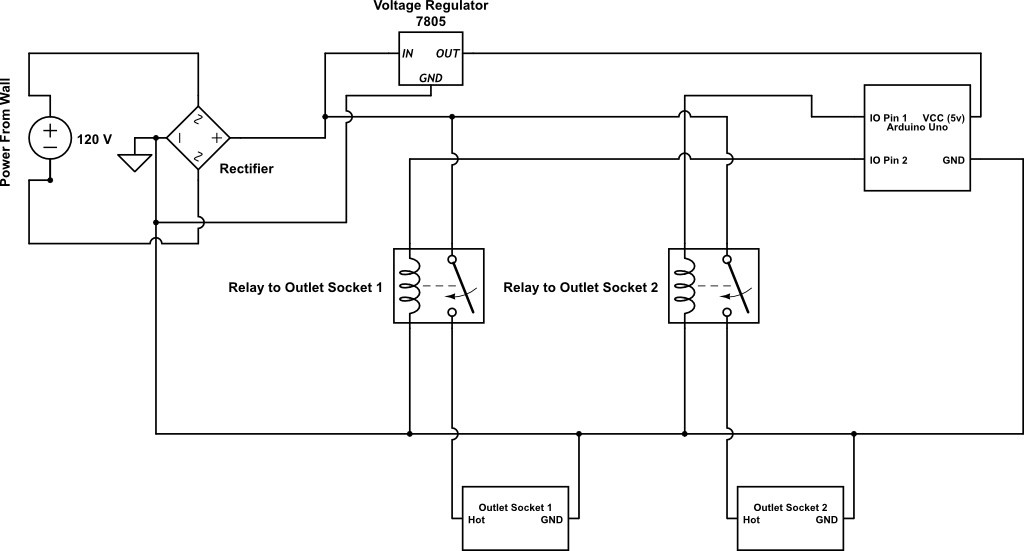
\includegraphics[width=0.9\columnwidth]{circuit}
\caption{Circuit design.}
\label{fig:circuit}
\end{figure}

\subsection {Functionality}
The deliverable of this project was an improved system that authorizes an outlet. It implemented all of the following optimizations described in the project description:
\begin{itemize}
\item A smaller form factor. Although never physically produced in this research, with proper equipment and skill set, this research’s design could allow for authorized power outlets to be contained in small wall warts. 
\item A wireless personal area network was created to allow for easy addition of outlets to existing infrastructure and freedom to put tools in areas far away from ethernet jacks. 
\item The controlled outlets automatically turn off after a period of inactivity to reduce the risk of unauthorized use of power outlets. 
\item The system can track usage of authorized devices by user.
\item Allowing users without NFC enabled devices to generate authorization requests by scanning a QR code placed on each connected device. 
\end{itemize}

\section{Discussion}
This research discovered many important improvements having to do with authorized power outlets. By demonstrating the ability to track usage of devices, these devices can not only take on the role of authentication but also as instruments of data collection. Additionally, finding a way to authenticate without NFC, QR in this case, indicates that the concept of authorized power outlets are adaptable to whatever type of authentication best suits its work environment. By proving that authorized power outlets can be organized into networks ran by base stations on a 1-N basis suggests that maybe these devices could experience the rapid growth wireless internet devices experienced when wireless routers became popular. 

This research also discovered some spots that might give authorized power outlet developers some trouble. In this research, it was a tremendous battle orienting the ZigBees in such a way that they would successfully communicate. If there was not a line of sight, the communication would very rarely work. Additionally, ZigBees operate at the 2.4GHz frequency, which is particularly saturated with other signals such as cordless phones, routers, etc. This can cause lots of interference.

Additionally, it is very hard to design printed circuit boards that are small enough to fit in a wall wart but big enough to fit all the necessary components. It also takes a special skill set and some special machinery to engineer a printed circuit board. Because of these setbacks, the research was not able to fully explore if it was possible to create a smaller form factor; however, progress was still made by creating a prototype in EAGLE CAD to help get the ball rolling with other research. Along with several attempts in printing this design to a physical circuit board resulted in poor traces and holes drilled at the wrong sizes.

All in all, the research garnered very exciting research to advance the concept of authorized power outlets in society.

\section{Future Work}
Looking ahead to the future, there are several opportunities for iteration and improvement upon the current advancements. Specifically, in the area of form factor, wireless radios, and auto-off functionality.

The highest priority is to continue developing a reduced form factor of the current outlet receptacle. Since the circuit design has already been completed, the most effort will be put into the actual printing of the circuit board and safely testing it. Reducing the size of the current form factor would increase the invisibility factor to the point where it could potentially just blend into an everyday environment increasing user adoption.

Experimenting with better radios could make the system more reliable, as the ZigBee’s are extremely prone to interference. This could further increase the range of communication between the receptacle outlets and the base station. 

The current, time based auto-off functionality has several flaws that leave room for improvement. Since the auto-off feature is time based, there must be a threshold time value set to turn off the powered device. Choosing this threshold could be difficult and may have to be done for each, individual device. This could also  lead to prematurely turning off a device while the user is actively using it. Therefore, an auto-off system implementing an anemometer may solve this problem. The anemometer could read how much current the machine was drawing and automatically turn the machine off if it is inactive for an extended period of time.

\section{Conclusion}
To improve on previous work on the authorized power outlets, several revisions were made to make the tool more scalable and usable. Alternative forms of authentication were used, such as QR codes, so that users not having NFC technologies in their mobile devices can also use the system. Also, in order to reduce risk of other users using the outlet, automatic timeout was added and thus, after a certain period of time, the tool will be turned off. Another helpful feature that was included in this revision was a system for tracking tool usage, which can help monitor the different tools in the lab and see which new tools need to be bought. Also, a smaller form factor was developed, which can make authorized power outlets more scalable. Finally, a wireless network was created so that outlets can be easily added.

All of these revisions has improved authorized power outlets and has made the system more easy to use. Allowing QR codes, having a wireless network, and making the system smaller allow for more scalability. The system can then incorporate many more devices and be more useful in the lab or at home. Improvements can be made to this system to incorporate more sophisticated ways to restrict access and track inactivity.

\section{References}
\begin{enumerate}
\item Fahsel, Michael. Personal Interview. 24 Feb 2013.

\item Fahsel, Ryan, Gray, Colin, and Ramakrishnan, Ramya. “NFC Authorized Outlet.” 2013.

\item Frankston, Bob. "(Not) in Control of Your Home [Bits Versus Electrons]."Consumer Electronics Magazine, IEEE 2.2 (2013): 56-58.

\item Heintzelman, Mike. Personal Interview. 1 Mar. 2013.

\item Myers, Jenny, and Jim Higgins. "Method and system for using wireless devices to control one or more generic systems." U.S. Patent Application 09/854,870.

\item Singhee, Mukul. "A framework for the design of systems with intelligent and interactive information flow." (2010).

\item Song, Guangming, et al. "A wireless power outlet system for smart homes."Consumer Electronics, IEEE Transactions on 54.4 (2008): 1688-1691.

\item Wicks, Angela M., John K. Visich, and Suhong Li. "Radio frequency identification applications in hospital environments." Hospital topics 84.3 (2006): 3-9.
\end{enumerate}

\section{Acknowledgments}

We thank Dr. Gregory D. Abowd, Dr. Thad Starner, Clint Zeagler, and Caleb Southern for leading the class Mobile and Ubiquitous Computing, which was the inspiration for this project.

% Balancing columns in a ref list is a bit of a pain because you
% either use a hack like flushend or balance, or manually insert
% a column break.  http://www.tex.ac.uk/cgi-bin/texfaq2html?label=balance
% multicols doesn't work because we're already in two-column mode,
% and flushend isn't awesome, so I choose balance.  See this
% for more info: http://cs.brown.edu/system/software/latex/doc/balance.pdf
%
% Note that in a perfect world balance wants to be in the first
% column of the last page.
%
% If balance doesn't work for you, you can remove that and
% hard-code a column break into the bbl file right before you
% submit:
%
% http://stackoverflow.com/questions/2149854/how-to-manually-equalize-columns-
% in-an-ieee-paper-if-using-bibtex
%
% Or, just remove \balance and give up on balancing the last page.
%
\pagebreak
\newpage
\section{Appendix A}

\begin{figure}[!h]
\centering
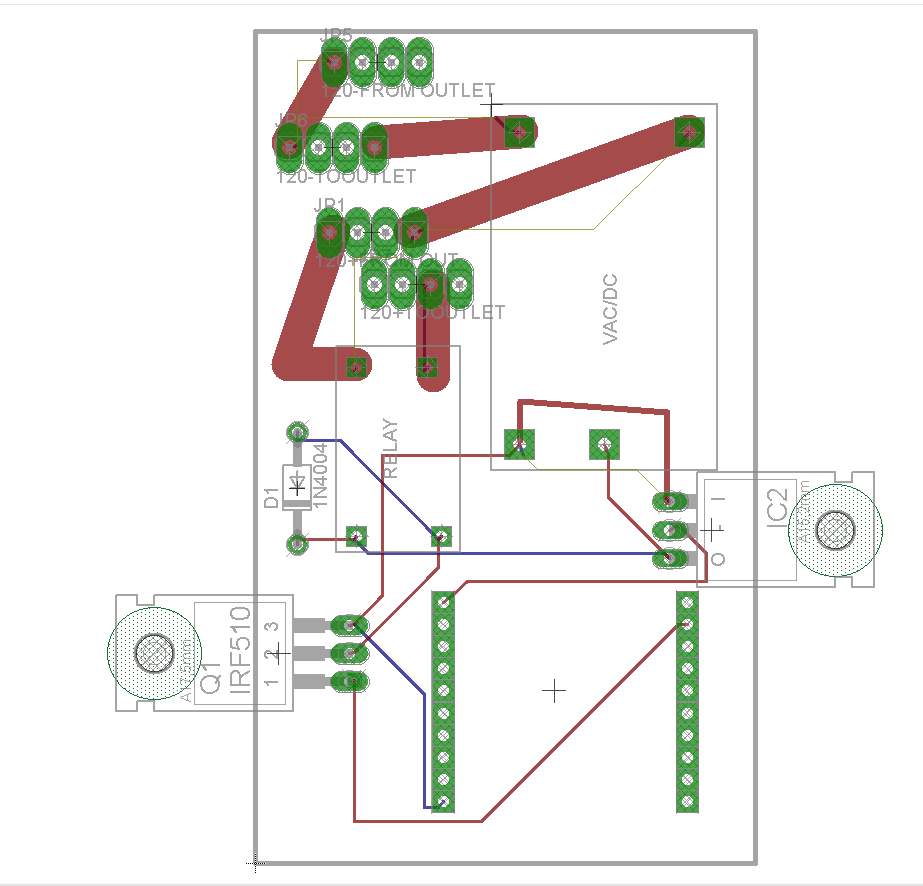
\includegraphics[width=0.9\columnwidth]{app_a}
\caption{EAGLE CAD circuit of small form factor printed circuit board.}
\label{fig:app_a}
\end{figure}

\section{Appendix B}

\begin{figure}[!h]
\centering
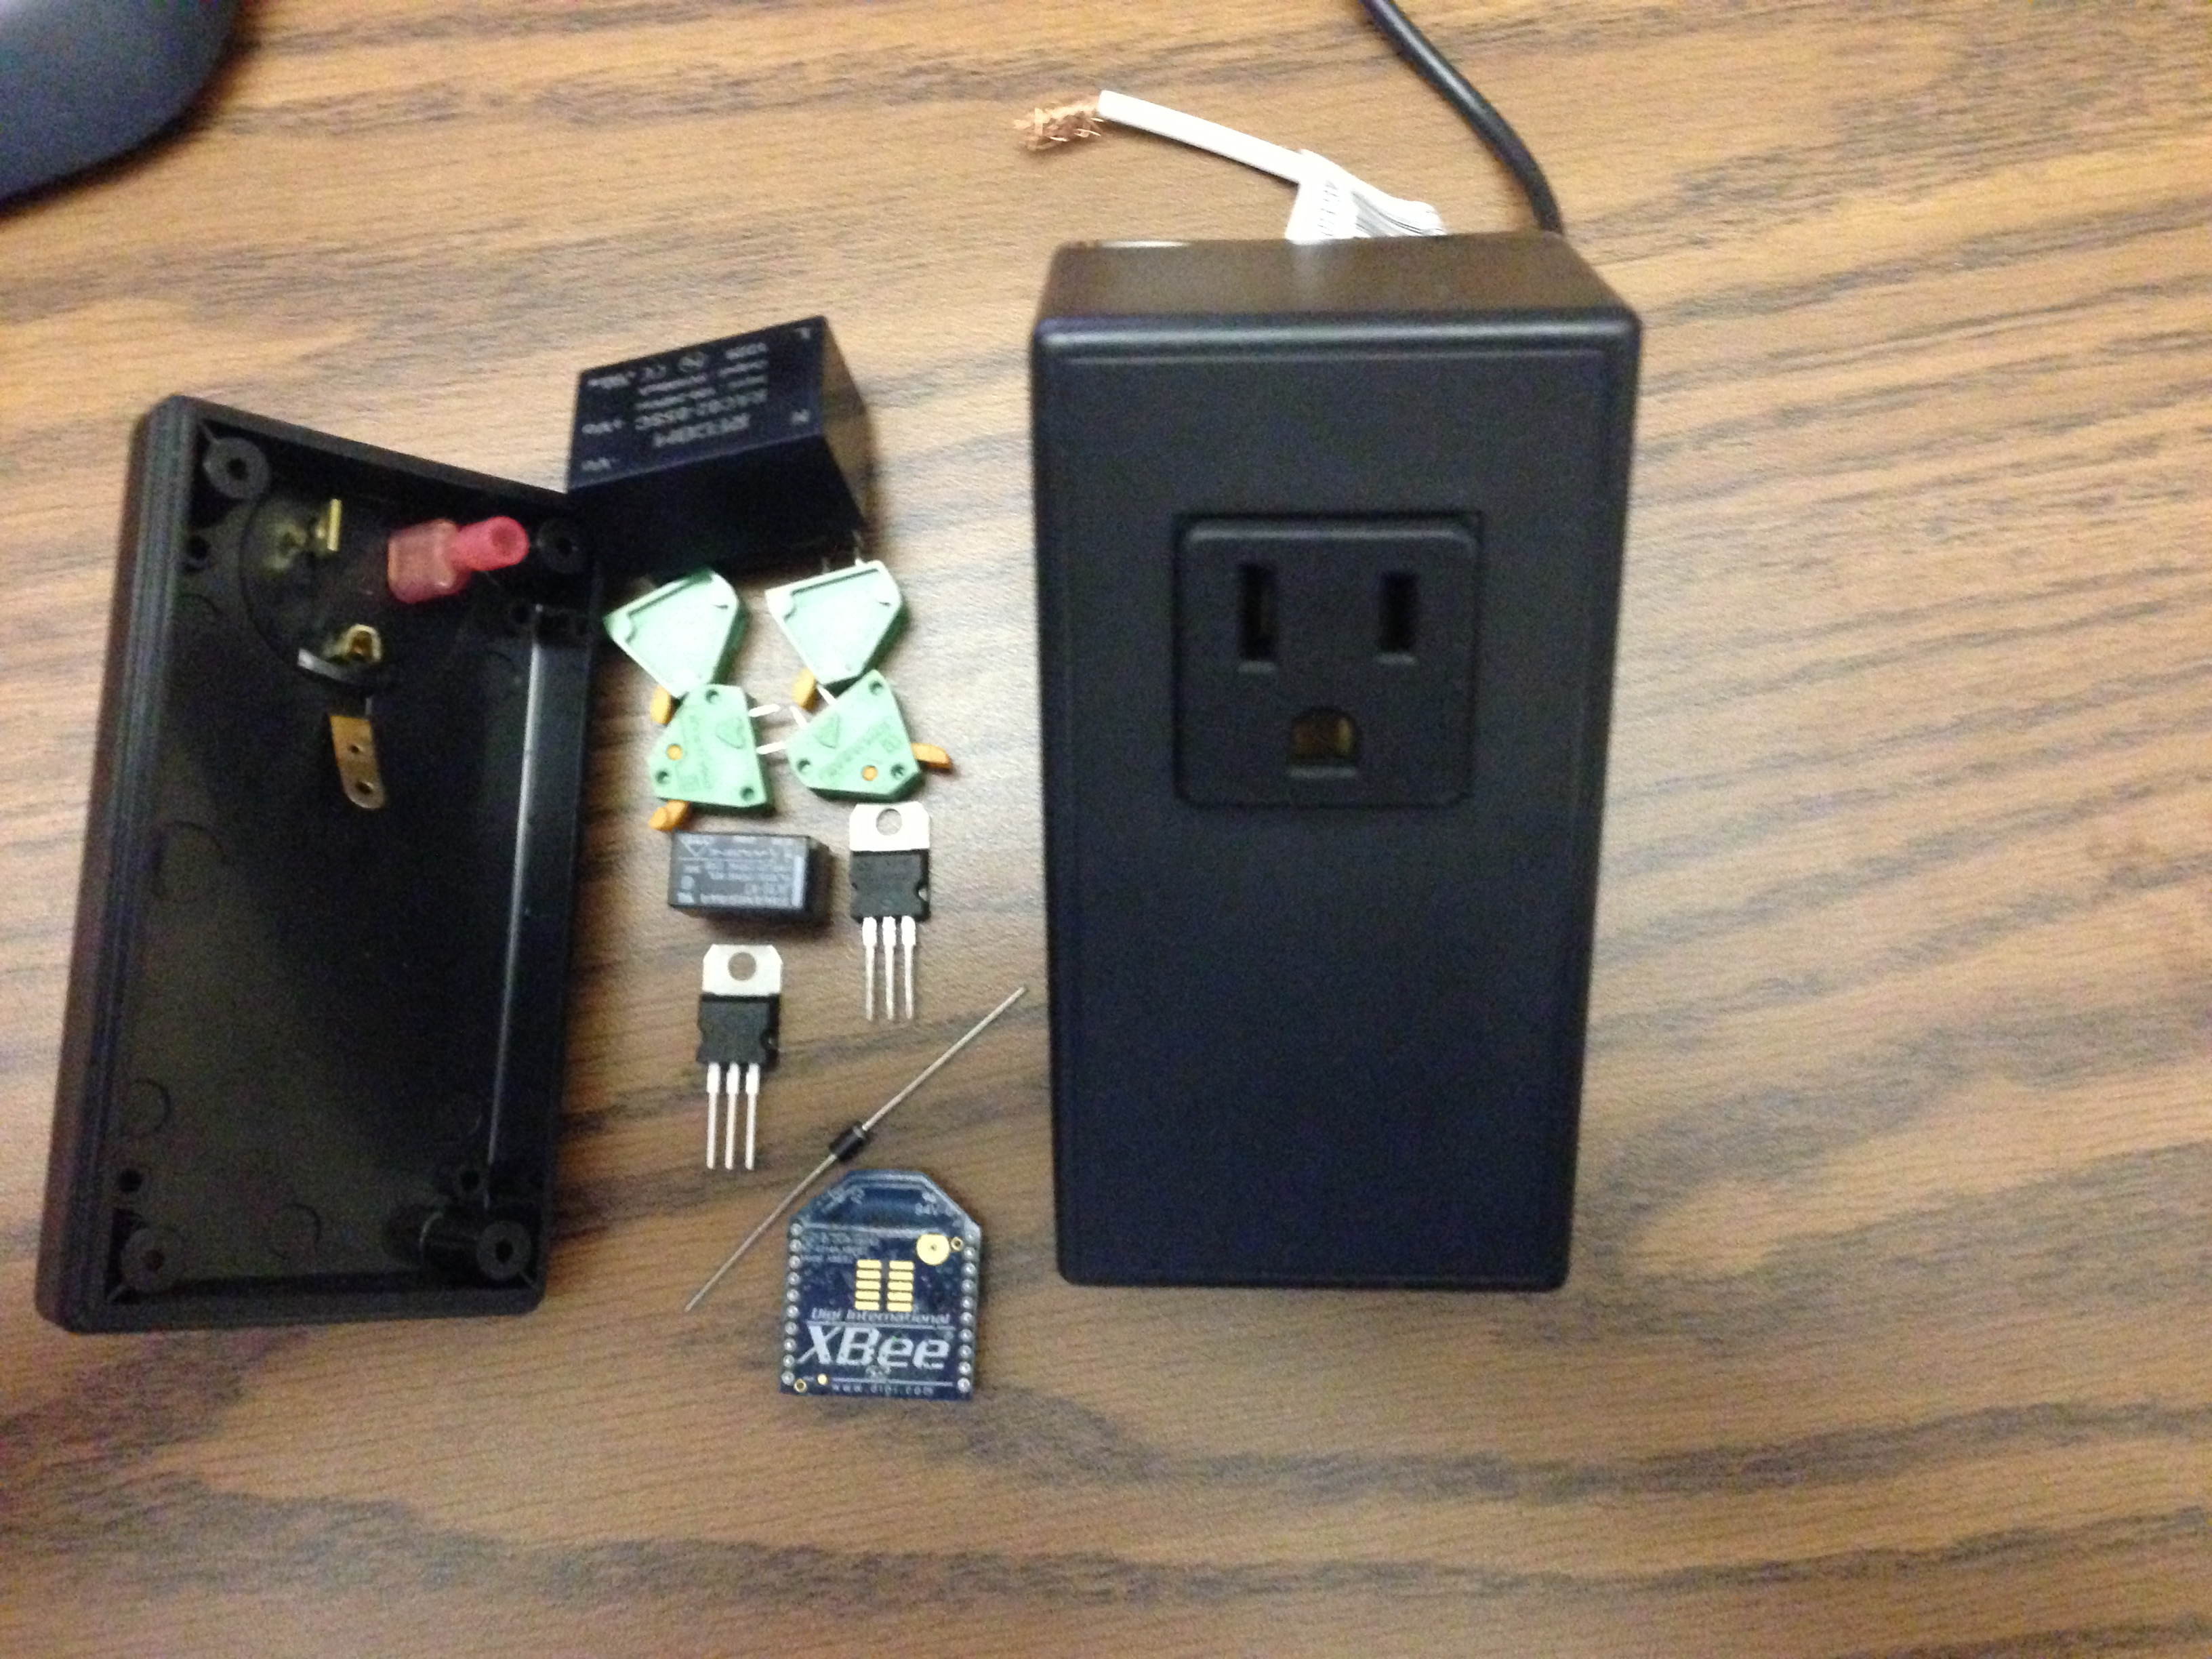
\includegraphics[width=0.9\columnwidth]{app_b}
\caption{Wall wart for small form factor.}
\label{fig:app_b}
\end{figure}
\newpage
\section{Appendix C}

\begin{figure}[!h]
\centering
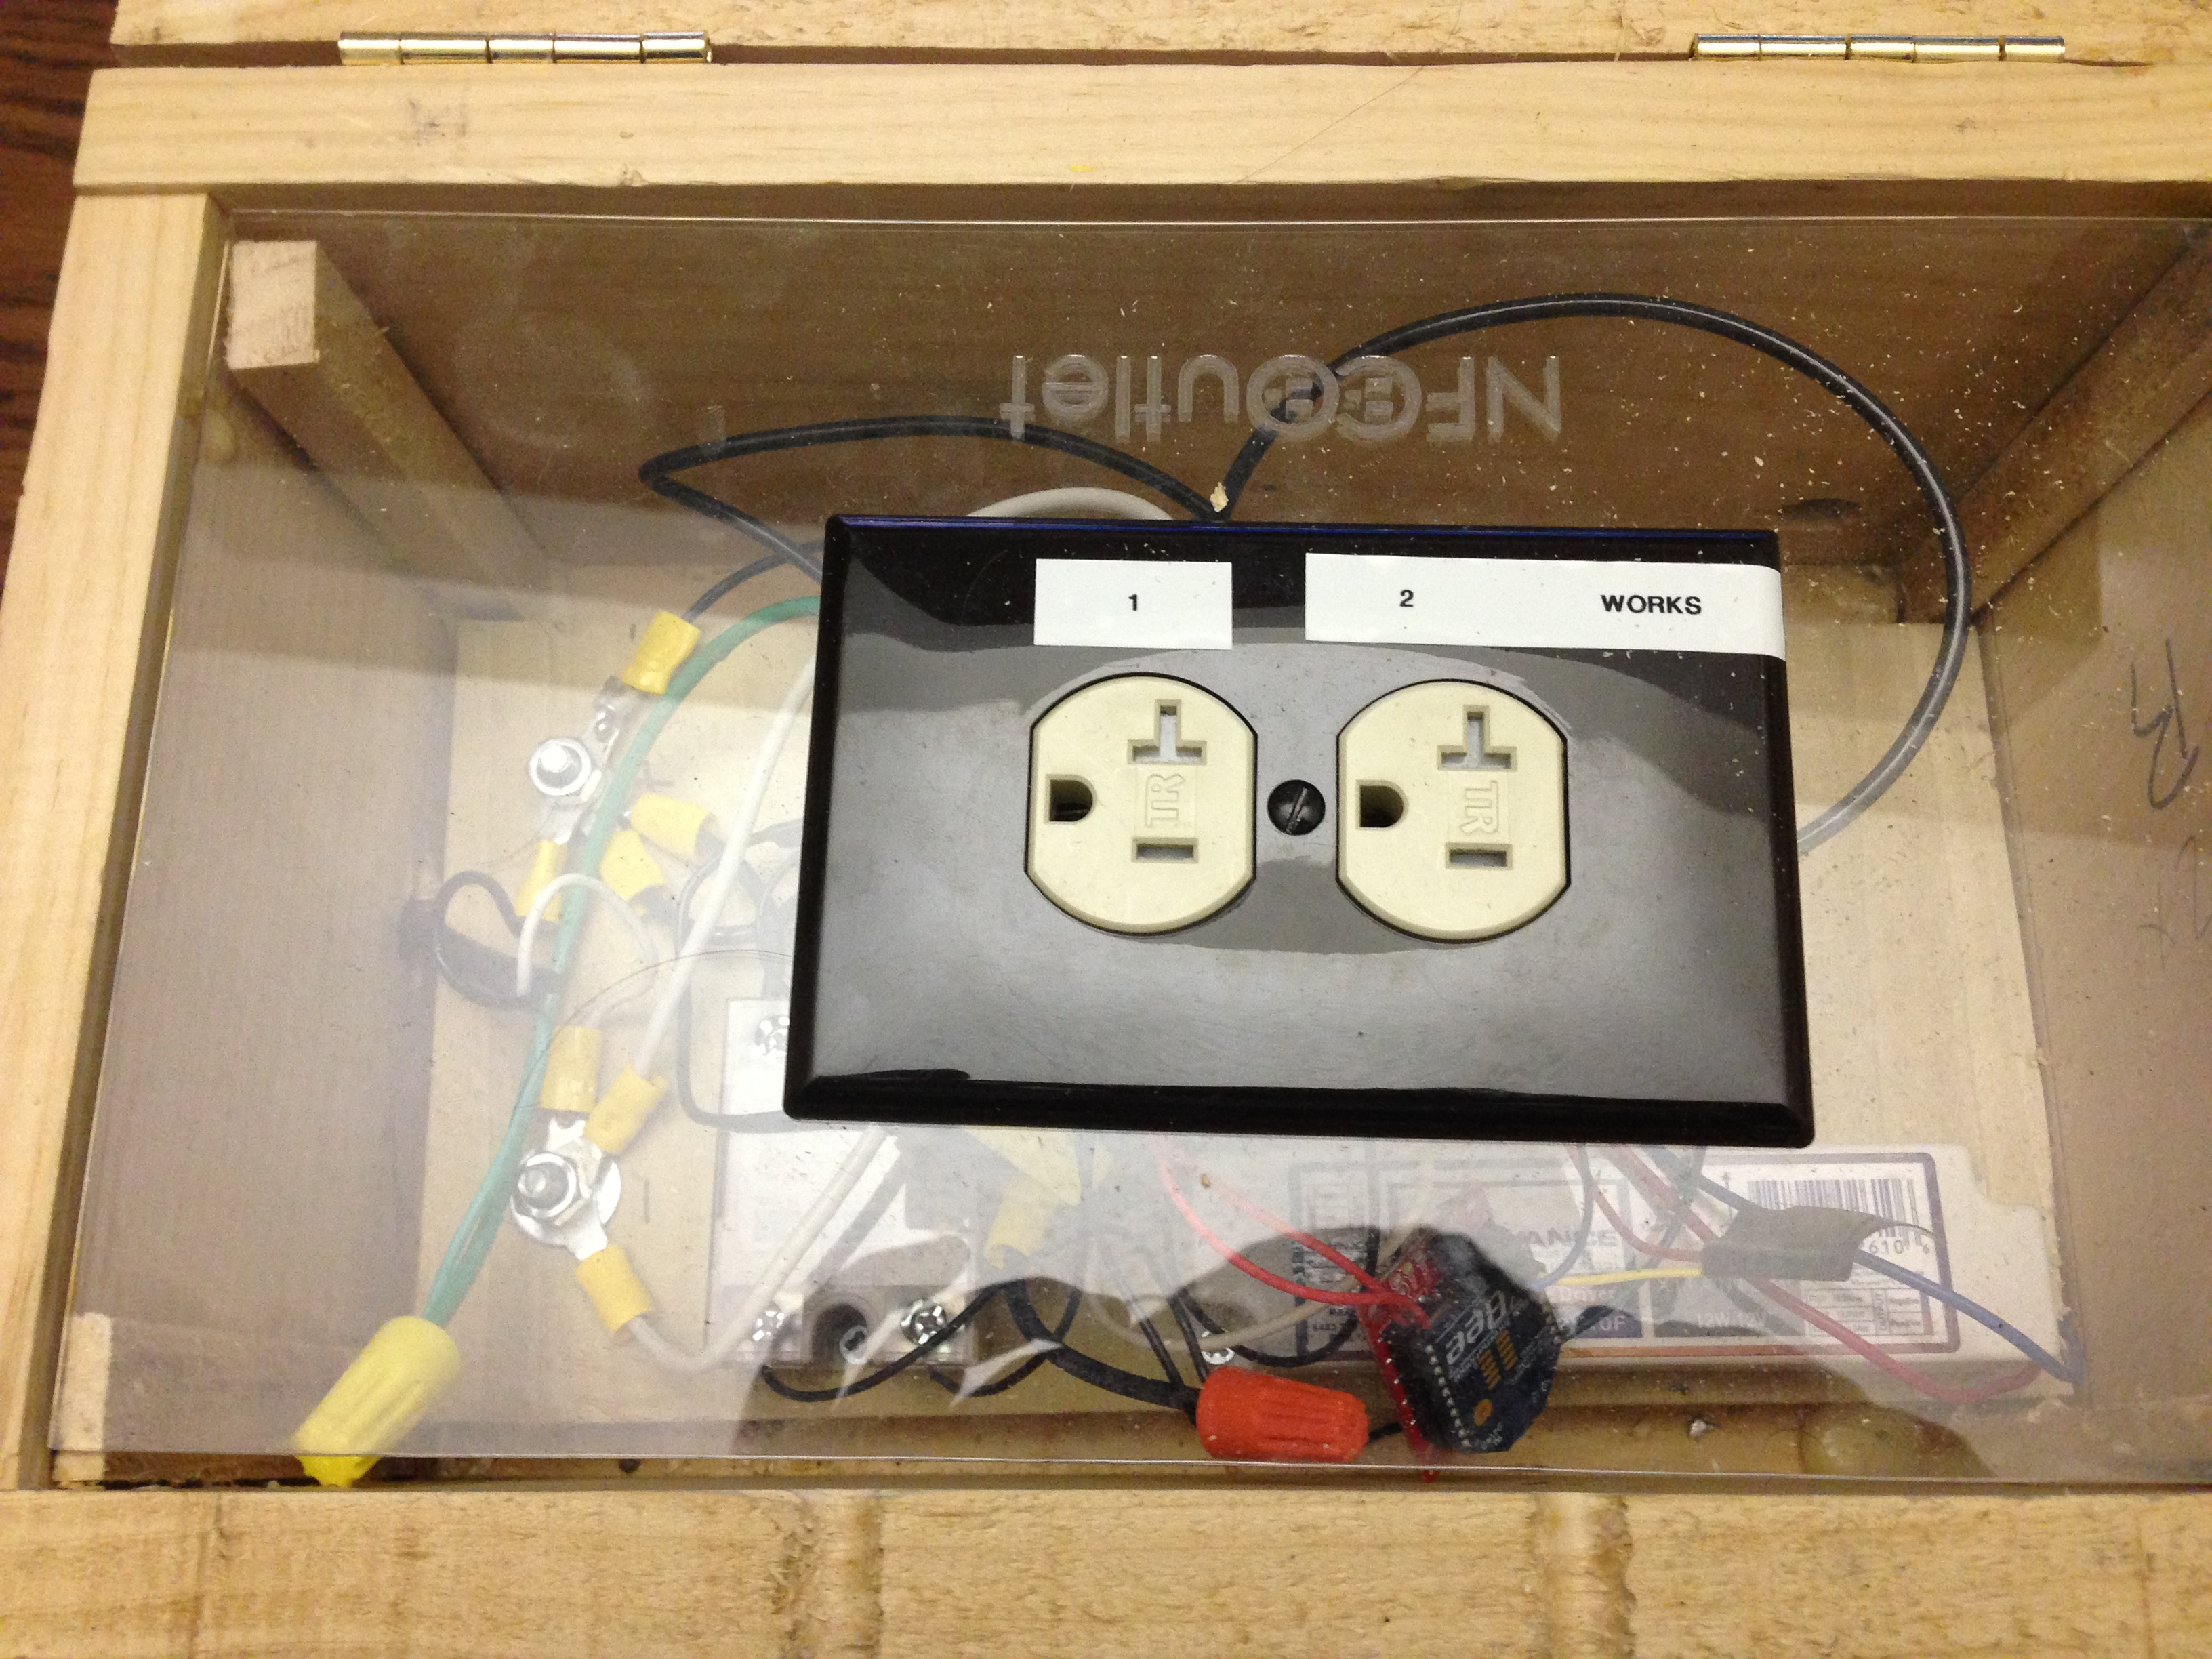
\includegraphics[width=0.9\columnwidth]{app_c}
\caption{Original NFCOutlet box with ZigBee instead of microcontroller.}
\label{fig:app_c}
\end{figure}

\section{Appendix D}

\begin{figure}[!h]
\centering
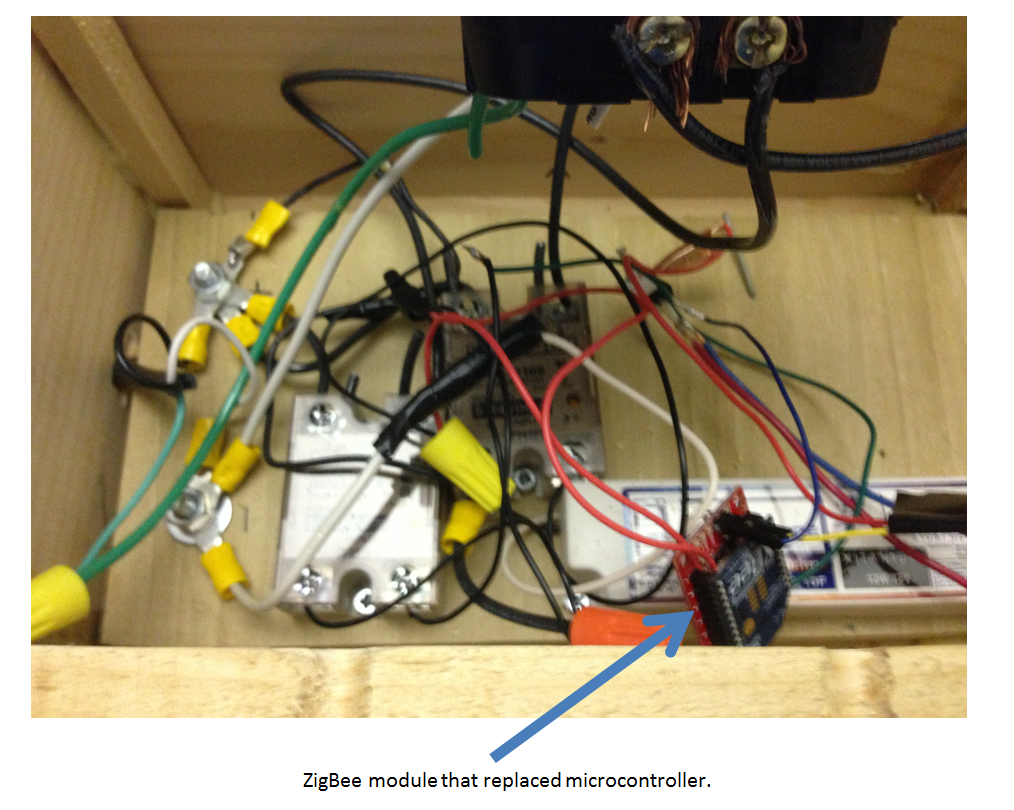
\includegraphics[width=0.9\columnwidth]{zig}
\caption{ZigBee located in NFCOutlet box.}
\label{fig:zig}
\end{figure}

%\balance

% If you want to use smaller typesetting for the reference list,
% uncomment the following line:
% \small
%\bibliographystyle{acm-sigchi}
%\bibliography{sample}
\end{document}
